\documentclass[journal]{IEEEtran}
\usepackage[T1]{fontenc}
\usepackage[utf8]{inputenc}
\usepackage{amsmath,amssymb,amsfonts}
\usepackage{graphicx}
\usepackage{booktabs}
\usepackage{multirow}
\usepackage{array}
\usepackage{cite}
\usepackage{url}
\usepackage{microtype}
\usepackage[hidelinks]{hyperref}
\graphicspath{{figures/}}

\hypersetup{
  pdftitle={A License-Clean Graph Neural Network for Fast Parasitic Extraction in PCB-Embedded Planar Magnetics: Numerical Fidelity, Symmetry, and Runtime Evaluation},
  pdfauthor={Duong Viet Hoang and Lun-Min Shih},
  pdfsubject={Graph-surrogate evaluation for PCB-embedded planar-magnetics parasitics}
}

\newcommand{\Cps}{C_{\mathrm{ps}}}
\newcommand{\Lp}{L_{\mathrm{p}}}
\newcommand{\Ls}{L_{\mathrm{s}}}
\newcommand{\Mut}{M}
\newcommand{\Rthree}{\mathrm{R3P16}}
\newcommand{\Rfour}{\mathrm{R4P16}}

\title{A License-Clean Graph Neural Network for Fast Parasitic Extraction in PCB-Embedded Planar Magnetics: Numerical Fidelity, Symmetry, and Runtime Evaluation}

\author{Duong Viet Hoang and Lun-Min Shih\\[-0.15ex]
\normalsize Department of Computer Science, Da-Yeh University, Taiwan\\[-0.15ex]
\normalsize Hoangduong4316@icloud.com, Lmshih@mail.dyu.edu.tw%
\thanks{This manuscript is Journal Snapshot 1 of the PCB Parasitic GNN research artifact. It extends an earlier conference-length snapshot while retaining version boundaries between numerical-reference packages.}}

\markboth{Journal Snapshot 1, September 2026}{Hoang and Shih: A License-Clean GNN for PCB Planar-Magnetics Parasitics}

\begin{document}
\maketitle

\begin{abstract}
PCB planar magnetics require rapid evaluation of winding capacitance and inductance, but a surrogate is useful only when its geometry, numerical references, evaluation split, and timing boundary are explicit. This work presents a license-clean, traceable graph-surrogate workflow for primary-to-secondary capacitance, primary and secondary free-space self-inductance, and mutual inductance. A shared geometry contract feeds graph construction, FastHenry, and a deterministic electrostatic finite-element implementation. The active corpus contains 1,500 synthetic active-leg layouts grouped into 66 swap-closed turn-count families. Across five family-held-out splits crossed with five initialization seeds, mean family-macro errors against the current numerical-reference package are 12.550, 4.173, 3.964, and 3.413 percent. The graph model has lower error than four frozen pooled-feature procedures in every matched cell and target, but this post-hoc comparison does not isolate graph connectivity. A controlled three-arm experiment does not establish a consistent gain from learned coordinate updates: all eight crossed-axis descriptive sensitivity intervals include zero. Encoded-graph symmetry checks pass within a tolerance of two times ten to the minus five. On a frozen 306-layout panel, the median paired ratio between the sequential FastHenry-plus-finite-element workflow and warm-loaded raw-record-to-four-output inference is 70,099-fold. These results measure agreement with fixed synthetic numerical references, not mesh-converged or fabricated-board accuracy.
\end{abstract}

\begin{IEEEkeywords}
finite-element method, graph neural network, parasitic extraction, planar magnetics, reproducibility, surrogate model.
\end{IEEEkeywords}

\section{Introduction}
\IEEEPARstart{P}{lanar} transformers and inductors replace wound wire with patterned copper conductors. Their compact geometry is useful in high-density converters, but broad conductor overlap and small inter-layer spacing make parasitic capacitance and inductive coupling sensitive to layer assignment, registration, and stackup~\cite{ouyang,hurley,mclyman,erickson}. These quantities influence common-mode current, leakage, ringing, and energy transfer~\cite{ott,paul}. Numerical extraction can resolve more geometry than compact formulas, yet repeated three-dimensional computation is expensive inside a design search.

A learned surrogate can reduce that cost, but three separable questions must be answered. First, do graph construction and the numerical solvers consume the same physical topology? Second, what numerical fidelity do the labels represent? Third, does an apparent speed or accuracy advantage survive a precisely stated split, uncertainty summary, and timing boundary? Treating a solver observation as physical truth, or comparing an in-memory neural forward pass with a vaguely defined solver time, obscures these questions.

This work therefore organizes the contribution as an evidence chain rather than a single headline model. A geometry contract rejects inconsistent layer heights, overlapping conductor volumes, out-of-board traces, duplicates, and passive-inductance violations before numerical labeling. FastHenry supplies the three free-space inductance targets~\cite{fasthenry}; a deterministic electrostatic volume finite-element method (FEM) supplies inter-winding capacitance. A message-passing graph neural network (GNN) predicts all four quantities. Family-held-out evaluation, fixed checkpoints, solver qualification, symmetry tests, and paired timing each have independent acceptance boundaries.

The principal contributions are:
\begin{itemize}
\item a 1,500-layout synthetic active-leg corpus with one shared geometry topology for graph, inductance, and capacitance computation;
\item explicit FEM domain, mesh-sensitivity, repeatability, and multi-fidelity results that prevent the bulk capacitance column from being called mesh-converged truth;
\item a complete five-by-five family-split and initialization grid for the current deterministic numerical-reference package;
\item fixed pooled-feature and coordinate-update controls that separate graph-level performance, coordinate updating, and encoded-graph symmetry; and
\item a paired all-four-target latency comparison from resident raw JSON through materialized outputs, together with its hardware and workflow limitations.
\end{itemize}

Fig.~\ref{fig:pipeline} summarizes the evidence path. Each reported number belongs to a versioned target package; older results are retained only when labeled with their original reference version.

\begin{figure*}[t]
\centering
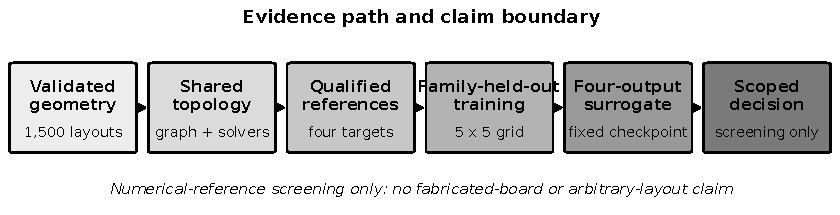
\includegraphics[width=\textwidth]{hoang1_pipeline.pdf}
\caption{Evidence path from geometry to a scope-qualified screening decision. The graph and both numerical solvers consume the same canonical conductor topology. Numerical-reference agreement is distinct from fabricated-board validation.}
\label{fig:pipeline}
\end{figure*}

\section{Motivation and Research Evolution}
\subsection{A Surrogate Inside the Design Loop}
Parasitic extraction is commonly invoked repeatedly rather than once. A designer changes conductor count, layer registration, spacing, or copper dimensions, re-extracts the parasitics, and then evaluates their circuit consequences. Full numerical solves remain valuable reference computations, but their latency limits broad screening and optimization. A learned map
\begin{equation}
\mathcal{S}_{\theta}:\mathcal{G}(\text{layout})\longrightarrow
[\Cps,\Lp,\Ls,\Mut]
\end{equation}
is therefore useful when it replaces repeated reference solves within a declared geometry domain. The intended role is screening: candidates selected by the surrogate still require higher-fidelity numerical analysis and, ultimately, measurement.

Accuracy and speed are inseparable from the definition of the map. A small prediction error is meaningful only relative to a named target package, while a runtime ratio is meaningful only when both paths produce the same target set and their included operations are stated. The present study treats geometry validity, reference fidelity, predictive agreement, symmetry, and latency as separate questions with separate evidence.

\subsection{From Feasibility Snapshot to Journal Study}
The earlier conference snapshot asked whether a graph surrogate could provide a rapid feasibility estimate for synthetic planar-magnetics geometries. That version remains an immutable record of its own data and timing boundaries. The journal study extends, rather than silently replaces, that work. It introduces a geometry-valid corpus, one topology shared by graph and solvers, deterministic capacitance generation, held-out turn-count families, a complete split-by-initialization grid, fixed comparison procedures, implementation-level symmetry checks, and a paired all-four-target timing estimand.

This evolution matters because a surrogate can faithfully learn a numerically generated target even when the target itself carries discretization error. For that reason, archived and current target-package results are never pooled. The earlier package is reported only as a version-sensitivity comparison; all current headline accuracy and runtime results use the deterministic FEM-v2 package.

\begin{figure*}[t]
\centering
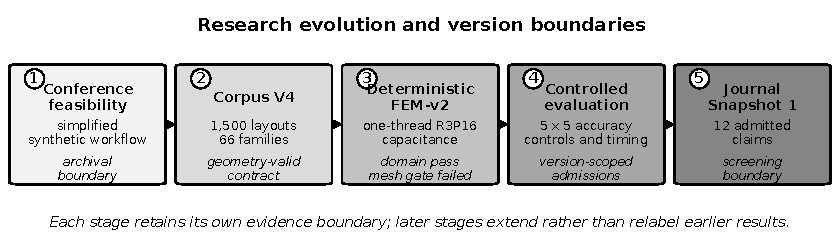
\includegraphics[width=\textwidth]{hoang9_research_evolution.pdf}
\caption{Research evolution and version boundaries. The conference package remains a feasibility-stage archive. Corpus V4 establishes the geometry contract; deterministic FEM-v2 defines the current capacitance package; controlled accuracy, baseline, coordinate-update, symmetry, and timing studies then support the journal snapshot. Later stages extend rather than relabel earlier evidence.}
\label{fig:research-evolution}
\end{figure*}

\subsection{License and Redistribution Boundary}
The repository distributes its original code, data-processing utilities, and manuscript assets under the BSD 3-Clause license. The GNN implementation uses plain PyTorch modules and does not require PyTorch Geometric or the Deep Graph Library. External numerical and machine-learning tools retain their own licenses and are not re-licensed or redistributed as project code. The packaged IEEEtran class retains its LaTeX Project Public License notice. The term \emph{license-clean} describes an explicit provenance and redistribution boundary; it is not a legal opinion and does not imply that every external solver binary or commercial geometry is bundled. All figures in this snapshot are generated from admitted project evidence rather than copied vendor artwork.

\section{Related Work}
\textit{Planar magnetics and parasitic models.}
Planar windings trade three-dimensional wire placement for lithographically
defined conductors, making stackup, registration, overlap, and interleaving
central design variables~\cite{ouyang,hurley,mclyman,erickson,kazimierczuk}.
Classical winding analysis remains indispensable for interpretation:
Dowell-type and related formulations explain frequency-dependent conductor
loss~\cite{dowell,ferreira}, while electromagnetic-compatibility treatments
connect common-mode current and coupling paths to system behavior~\cite{ott,paul}.
Those works motivate the target quantities, but they do not make a compact
formula an interchangeable reference for every three-dimensional layout.

\textit{PEEC, inductance, and capacitance extraction.}
The partial-element equivalent-circuit formulation maps field interactions to
circuit quantities~\cite{ruehli}; Grover's formulas provide useful closed-form
inductance estimates~\cite{grover}. FastHenry instead constructs a
three-dimensional partial-inductance system and accelerates its solution with
multipole methods~\cite{fasthenry}. FastCap applies the same broad computational
idea to boundary-integral capacitance extraction~\cite{fastcap}, building on
adaptive multipole and preconditioned integral-equation techniques
~\cite{carrier88,nabors94}. These methods define numerical observations under a
specific geometry, discretization, and port composition. Agreement with such an
observation is therefore different from agreement with a manufactured device.

\textit{FEM implementation and discretization evidence.}
Standard finite-element theory separates algebraic-solver error from
discretization error~\cite{brenner}. Conjugate gradients, multilevel
preconditioners, and scalable scientific-software interfaces address the former
~\cite{hestenes,hypre,petsc}; geometry and assembly packages provide practical
meshing and weak-form infrastructure~\cite{gmsh,skfem}. Mesh adequacy requires
its own evidence. Adaptive marking and recovery-based a posteriori estimators
are established routes to controlling discretization error
~\cite{doerfler,zienkiewicz}. The present study does not claim such an estimator:
it reports a predeclared adjacent-mesh test, preserves its negative outcome,
and names both retained fidelities.

\textit{Graph learning and learned physics.}
Graph convolution and message passing encode relational inductive biases
~\cite{kipf,gin,gilmer,battaglia}; the implementation here uses the PyTorch
autodifferentiation stack and a fixed AdamW optimization schedule
~\cite{pytorch,adamw}. Continuous-filter and directional molecular networks show
how distance and angular structure can enter graph messages
~\cite{schnet,dimenet}. Learned graph simulators operate on particles or meshes
~\cite{sanchez,pfaff}, while neural operators and physics-informed networks
learn functions or fields rather than only lumped outputs
~\cite{fno,deeponet,pinn}. This work takes the narrower scalar-surrogate route:
the field solvers remain outside the model, and the network predicts four
declared numerical-reference quantities.

\textit{Equivariance.}
Tensor Field Networks, SE(3)-Transformers, PaiNN, EGNN, and NequIP illustrate
distinct ways of imposing geometric transformation laws
~\cite{tfn,se3transformer,painn,egnn,nequip}. Their results motivate
symmetry-aware architectures but do not imply that a coordinate-update branch
must improve every scalar task. Here the algebraic statement is limited to the
already encoded graph, numerical transformation tests verify the executed
implementation, and a separate fixed-budget ablation asks whether learned
coordinate updates improve the four target errors.

\textit{Machine learning in EDA.}
Machine learning now supports multiple stages of electronic design automation
~\cite{huang_survey}. Prior graph-based work addresses layout parasitics,
distributed circuits, chip placement, transistor sizing, and pre-placement
wirelength~\cite{paragraph,circuitgnn,mirhoseini,gcnrl,net2}; CircuitNet provides
an open benchmark for several physical-design prediction tasks
~\cite{circuitnet}. These studies establish that circuit and layout structure
can be represented relationally. The present setting differs in its coupled
PCB-winding targets, solver-defined fidelity boundary, geometry-family split,
and paired all-four-target timing estimand.

\textit{Benchmarking, uncertainty, and reproducibility.}
Ridge regression, Random Forests, and Extremely Randomized Trees provide
well-defined non-graph controls~\cite{ridge,randomforest,extratrees}. Model
comparison is nevertheless sensitive to resampling dependence, finite test
sets, and multiple data sets~\cite{nadeau,varoquaux,demsar}. Bootstrap
resampling is a descriptive tool whose interpretation depends on the sampling
unit~\cite{efron}. Reproducibility guidance further motivates explicit code,
data, and reporting boundaries~\cite{pineau}. Finally, computer-experiment and
surrogate-model literature distinguishes emulator error, calibration, design
coverage, and global sensitivity~\cite{sacks,kennedy,queipo,saltelli}. Following
that distinction, this paper reports seed-grid and family-cluster sensitivity
ranges as descriptive intervals without a population-coverage interpretation, and
keeps numerical-reference agreement separate from physical calibration.

The contribution is therefore not a new field solver or a claim of hardware
calibration. It is an integrated audit of geometry validity, solver fidelity,
graph prediction, encoded-graph symmetry, controlled model comparisons, and
paired runtime on one versioned synthetic benchmark.

\section{Problem Formulation and Parasitic Theory}
\subsection{Two-Winding Target System}
For winding currents $\mathbf{i}=[i_{\mathrm{p}},i_{\mathrm{s}}]^{T}$, the free-space winding inductance matrix is
\begin{equation}
\mathbf{L}_{\mathrm{w}}=
\begin{bmatrix}
\Lp & \Mut\\
\Mut & \Ls
\end{bmatrix},
\qquad
W_{\mathrm{m}}=\frac{1}{2}\mathbf{i}^{T}\mathbf{L}_{\mathrm{w}}\mathbf{i}.
\label{eq:energy_inductance}
\end{equation}
Passivity requires $\mathbf{L}_{\mathrm{w}}$ to be positive semidefinite, hence $\Lp\geq0$, $\Ls\geq0$, and
\begin{equation}
|\Mut|\leq\sqrt{\Lp\Ls}.
\label{eq:passivity}
\end{equation}
The fourth target, $\Cps$, is a two-terminal electrostatic capacitance between the conductor groups. The learning problem is to estimate
\begin{equation}
\mathbf{y}=[\Cps,\Lp,\Ls,\Mut]
\end{equation}
from a canonical conductor graph while preserving finite, positive self quantities and the physical scope of the numerical references.

\subsection{Partial Inductance and Winding Composition}
At angular frequency $\omega$, the conductor-port impedance can be written
\begin{equation}
\mathbf{Z}(\omega)=\mathbf{R}(\omega)+j\omega\mathbf{L}(\omega),
\qquad
\mathbf{L}(\omega)=\frac{\operatorname{Im}\mathbf{Z}(\omega)}{\omega}.
\label{eq:partial_matrix}
\end{equation}
Let $\mathbf{a}_{\mathrm{p}}$ and $\mathbf{a}_{\mathrm{s}}$ encode the signed series connection of primary and secondary trace segments. The winding quantities follow by projection,
\begin{align}
\Lp&=\mathbf{a}_{\mathrm{p}}^{T}\mathbf{L}\mathbf{a}_{\mathrm{p}}, &
\Ls&=\mathbf{a}_{\mathrm{s}}^{T}\mathbf{L}\mathbf{a}_{\mathrm{s}},\nonumber\\
\Mut&=\mathbf{a}_{\mathrm{p}}^{T}\mathbf{L}\mathbf{a}_{\mathrm{s}}.
\label{eq:winding_projection}
\end{align}
This form makes current orientation explicit and generalizes the entrywise self-plus-mutual sums used by the implemented series convention.

\subsection{Electrostatic Capacitance}
Let $\Omega$ be the padded dielectric domain after conductor volumes are removed. With fixed potentials on the two winding surfaces, the weak electrostatic problem seeks $\phi$ such that
\begin{equation}
\int_{\Omega}\epsilon\nabla\phi\cdot\nabla v\,\mathrm{d}\Omega=0
\label{eq:electrostatic_weak}
\end{equation}
for every admissible test function $v$ that vanishes on the Dirichlet boundaries. For winding potential difference $\Delta V$, the field energy and extracted capacitance are
\begin{equation}
W_{\mathrm{e}}=\frac{1}{2}\int_{\Omega}\epsilon|\nabla\phi|^{2}\,\mathrm{d}\Omega,
\qquad
\Cps=\frac{2W_{\mathrm{e}}}{(\Delta V)^{2}}.
\label{eq:cap_energy}
\end{equation}
Equations~\eqref{eq:electrostatic_weak} and \eqref{eq:cap_energy} show why domain truncation and mesh resolution are properties of the capacitance target, not of the GNN.

\section{Shared Geometry and Dataset Contract}
\subsection{Active-Leg Geometry}
Each layout contains rectangular copper traces with net, layer, center coordinate, width, length, thickness, conductivity, and dielectric metadata. The current corpus comprises 1,500 unique layouts in 66 swap-closed turn-count families. Graph construction, FastHenry, and FEM receive the same conductor boxes, centers, and identities. Fig.~\ref{fig:geometry} shows the abstraction and its exclusions.

\begin{figure*}[t]
\centering
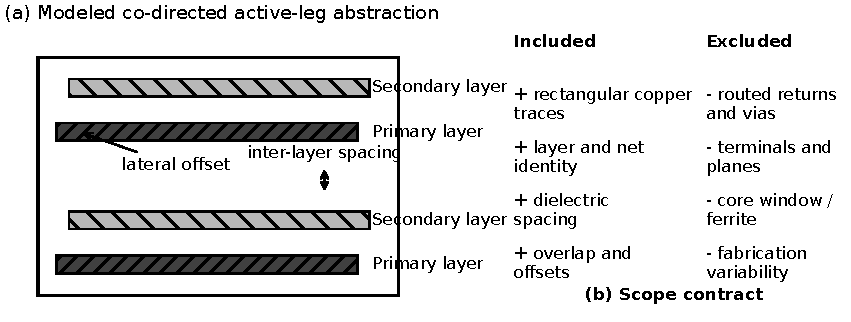
\includegraphics[width=\textwidth]{hoang2_geometry_scope.pdf}
\caption{Synthetic geometry scope. The corpus varies active-leg conductor placement and stackup quantities but does not contain complete routed windings, returns, vias, terminals, planes, the ferrite window, or manufacturing variability.}
\label{fig:geometry}
\end{figure*}

The geometry is intentionally narrower than a manufactured transformer. Co-directed active legs expose conductor count, inter-layer distance, overlap, and registration while avoiding an unverified reconstruction of returns and terminals. Consequently, the corpus supports numerical-reference screening experiments, not arbitrary-PCB or fabricated-device accuracy.

\subsection{Canonicalization and Acceptance Gates}
Every trace record is canonicalized before graph construction or solver export. The stored vertical coordinate must agree with the declared layer and stackup; conductor boxes must remain inside the board envelope and must not occupy overlapping volume; records must be unique; and numerical targets must be finite and satisfy~\eqref{eq:passivity}. Rejection occurs before a layout can enter a training or evaluation registry. This contract prevents the graph and field solvers from interpreting two different physical layouts under one identifier.

The current data generator varies turn count, conductor dimensions, layer allocation, spacing, registration, conductivity, and dielectric descriptors within a frozen active-leg grammar. Families are indexed by the primary and secondary turn-count pair and closed under winding-label swap. A family-held-out split therefore removes the complete turn-count family rather than randomly separating nearby instances of the same family.

The model does not predict nonlinear core magnetization, frequency-dependent permeability, copper loss, or a broadband RLGC matrix. Nor does the active-leg geometry represent routed return conductors, vias, terminals, planes, or the ferrite window. These omissions define the scientific boundary of the current benchmark rather than hidden deployment assumptions.

\section{Numerical Reference Construction}
\subsection{Inductance}
FastHenry evaluates the conductor system at 100~kHz and returns the complex port response from which the partial-inductance matrix in~\eqref{eq:partial_matrix} is obtained. Each canonical trace box is emitted as a finite-conductivity conductor with the same centerline, cross section, and net identity used by graph construction. The signed series vectors in~\eqref{eq:winding_projection} then produce the three winding targets. Finite and passive winding compositions are required. An independent Neumann-integral route is retained as an implementation cross-check rather than a claim of identical discretization. Solver agreement establishes numerical consistency, not fabricated-board truth.

\subsection{Electrostatic FEM}
The capacitance reference solves
\begin{equation}
\nabla\cdot(\epsilon\nabla\phi)=0
\end{equation}
on a padded three-dimensional domain, with opposite winding conductor groups assigned fixed potentials. Piecewise finite-element basis functions convert~\eqref{eq:electrostatic_weak} into
\begin{equation}
\mathbf{K}\boldsymbol{\varphi}=\mathbf{b},
\qquad
K_{ab}=\int_{\Omega}\epsilon\nabla N_a\cdot\nabla N_b\,\mathrm{d}\Omega,
\label{eq:fem_system}
\end{equation}
after applying the Dirichlet constraints. The discrete field energy yields the two-terminal capacitance through~\eqref{eq:cap_energy}. A direct solve and an algebraic-multigrid-preconditioned conjugate-gradient solve reproduce the same diagnostic linear system within the declared residual tolerance. This qualifies the backend implementation but is not independent physical validation.

Two named fidelities are retained. FEM-$\Rthree$ is the deterministic bulk target, with refinement level 3 and 16~mm domain padding. FEM-$\Rfour$ is a higher-resolution comparator on a selected registry. Neither is called continuum truth.

The numerical program therefore separates three questions. Domain sensitivity tests whether the artificial exterior boundary is sufficiently remote on a frozen panel. Adjacent-mesh sensitivity measures the change induced by one refinement step. Repeatability tests whether repeated executions reproduce the mesh and capacitance under a fixed software and threading configuration. Passing one gate does not imply passing either of the others.

For an ordered pair of numerical settings $A$ and comparator $B$, the reported design-level change is
\begin{equation}
\delta(A,B)=100\frac{|C_A-C_B|}{|C_B|}\ \%.
\label{eq:fidelity_delta}
\end{equation}
The domain comparison takes refinement-3 with 12~mm padding as $A$ and refinement-3 with 16~mm padding as $B$. The mesh comparison takes refinement-3 as $A$ and refinement-4 as $B$, both at 16~mm padding. Median and maximum values are evaluated against the predeclared 2% and 5% gates. A passed gate means only that the measured panel and perturbation satisfy those thresholds; it is not a statement of exactness.

\subsection{Domain, Mesh, and Repeatability Gates}
Nine layouts were selected by crossing trace-count strata with low, median, and high capacitance order statistics. At refinement 3, expanding the domain from 12 to 16~mm changes capacitance by a median 0.189658\% and a maximum 2.491566\%, passing the predeclared 2\% median and 5\% maximum gates. At 16~mm padding, refinement 3 versus 4 differs by a median 8.273879\% and a maximum 13.886399\%, failing those gates. Thus the bulk target is domain-qualified on the tested panel but not mesh-converged.

A separate three-layout, five-repeat panel exposed a thread-sensitive meshing path. The earlier 25-thread configuration failed mesh identity and a $10^{-4}$ capacitance-repeatability gate on all three layouts, with relative spreads from $5.59\times10^{-4}$ to $7.42\times10^{-3}$. The deterministic one-thread path passed both gates on all three, with maximum spread $8.45\times10^{-15}$. The deterministic path defines the current FEM-v2 target package; this result does not retroactively validate the older labels.

\begin{figure*}[t]
\centering
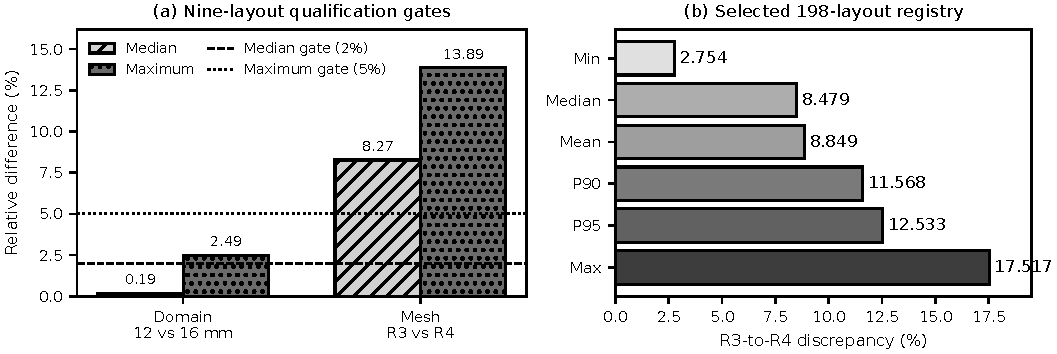
\includegraphics[width=\textwidth]{hoang3_fem_fidelity.pdf}
\caption{Capacitance fidelity evidence. (a) Domain expansion passes while the adjacent-mesh comparison fails. (b) On the deterministic 198-layout registry, every R3 observation exceeds its paired R4 observation; the summaries describe this selected panel rather than a population.}
\label{fig:fidelity}
\end{figure*}

On a deterministic registry of 198 layouts, with three from each of 66 families, every FEM-$\Rthree$ value exceeds its paired FEM-$\Rfour$ value. The median relative discrepancy is 8.479\%, with an observed range of 2.754\% to 17.517\%. Nine entries inherit the label-informed convergence selection; the other 189 are geometry-only selections. No inferential interval, global correction, or continuum-error interpretation is attached.

\section{Graph Surrogate}
\subsection{Representation and Prediction}
Each trace becomes a node in $\mathcal{G}=(\mathcal{V},\mathcal{E})$. The node stores its center $\mathbf{x}_i$ together with dimensions, logarithmic conductivity, dielectric descriptors, and normalized layer index. Edge state $\mathbf{a}_{ij}$ contains relative displacement, distance, overlap, layer separation, and a relationship type derived from the winding identities. A generic message-passing layer is
\begin{align}
\mathbf{m}_{ij}^{(\ell)}&=\phi_{e}^{(\ell)}\!\left(\mathbf{h}_{i}^{(\ell)},
\mathbf{h}_{j}^{(\ell)},\mathbf{a}_{ij},r_{ij}^{2}\right),\nonumber\\
\overline{\mathbf{m}}_{i}^{(\ell)}&=\operatorname*{AGG}_{j:(i,j)\in\mathcal{E}}
\mathbf{m}_{ij}^{(\ell)},\nonumber\\
\mathbf{h}_{i}^{(\ell+1)}&=\phi_{h}^{(\ell)}\!\left(
\mathbf{h}_{i}^{(\ell)},\overline{\mathbf{m}}_{i}^{(\ell)}\right),
\label{eq:message_passing}
\end{align}
where $r_{ij}^{2}=\|\mathbf{x}_{i}-\mathbf{x}_{j}\|_{2}^{2}$ and aggregation is permutation invariant. Four layers propagate pairwise conductor context. Mean, maximum, and log-compressed sum pooling retain complementary intensive, extreme, and size-sensitive graph summaries; a regression head materializes all four targets~\cite{gilmer}.

For each positive target $y_q$, training uses a train-only standardized logarithmic coordinate
\begin{equation}
z_q=\frac{\log(1+y_q)-\mu_q}{\sigma_q}.
\label{eq:target_transform}
\end{equation}
The optimization objective is the mean smooth-$L_1$ loss across the four standardized targets. Inference applies the frozen inverse transform and rejects nonfinite outputs. AdamW optimization uses a fixed 200-epoch budget~\cite{adamw}; validation loss is diagnostic and does not choose the checkpoint.

\subsection{Coordinate Updates and the Symmetry Boundary}
The baseline graph surrogate uses absolute and relative geometric features. A separate distance-message network computes scalar messages from invariant inputs and applies the coordinate update
\begin{equation}
\mathbf{x}_{i}^{(\ell+1)}=\mathbf{x}_{i}^{(\ell)}+
\frac{1}{|\mathcal{N}(i)|}\sum_{j\in\mathcal{N}(i)}
\frac{\mathbf{x}_{i}^{(\ell)}-\mathbf{x}_{j}^{(\ell)}}{1+r_{ij}^{(\ell)}}
\phi_x^{(\ell)}\!\left(\mathbf{m}_{ij}^{(\ell)}\right).
\label{eq:coordinate_update}
\end{equation}
Under the Euclidean action
\begin{equation}
\mathbf{x}'_i=\mathbf{Q}\mathbf{x}_i+\mathbf{t},\qquad \mathbf{Q}^{T}\mathbf{Q}=\mathbf{I},
\label{eq:e3_action}
\end{equation}
squared distances and scalar messages remain unchanged. Relative vectors transform as $\mathbf{Q}(\mathbf{x}_{i}-\mathbf{x}_{j})$, so every summand in~\eqref{eq:coordinate_update} transforms by $\mathbf{Q}$ and translation cancels. Induction over layers gives $\mathbf{x}_{i}'^{(\ell)}=\mathbf{Q}\mathbf{x}_{i}^{(\ell)}+\mathbf{t}$, while permutation-invariant pooling gives an invariant scalar output. The executed coordinate path is therefore $E(3)$-equivariant in its coordinates and invariant in its predicted scalars on encoded graphs. This conclusion does not apply automatically to arbitrary rotations of raw layout files because fixed axis-aligned overlap metadata is computed before the group action.

\begin{figure*}[t]
\centering
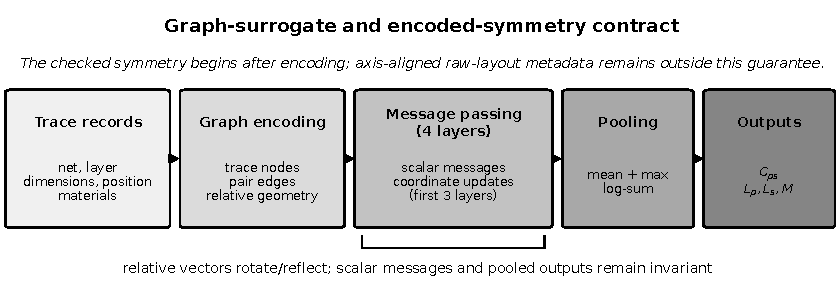
\includegraphics[width=\textwidth]{hoang8_graph_contract.pdf}
\caption{Graph-surrogate and symmetry contract. Canonical trace records form a relational graph; four distance-message layers feed mean, maximum, and log-compressed sum pooling and a four-output head. The coordinate-update branch is equivariant on encoded graphs, while scalar outputs are invariant. Fixed axis-aligned metadata limits extension to arbitrary rotations of raw layout files.}
\label{fig:graph-contract}
\end{figure*}

\subsection{Implementation Symmetry Checks}
The initialized coordinate-update implementation was evaluated on 200 transformed encoded graphs. Maximum scalar-output and coordinate residuals are $3.919\times10^{-7}$ and $1.407\times10^{-7}$, below the $2\times10^{-5}$ tolerance. In the trained three-arm study, all 75 checkpoints pass 40 transforms on seven validation-family fixtures, including translations, proper and improper orthogonal transforms, and node permutations. Across 21,000 graph-transform evaluations, the largest scalar residual among the three arms is $4.043\times10^{-7}$ and the moving-coordinate equivariance residual is $2.739\times10^{-7}$. These finite floating-point checks establish an implementation property on encoded graphs; they are not a formal proof for every possible raw layout.

\section{Evaluation Protocol}
\subsection{Family-Held-Out Grid}
The 66 turn-count families are partitioned into five deterministic held-out panels. Each split holds out 13 complete swap-closed families and contains 282 to 306 layouts. Five initialization seeds are crossed with the five split seeds, yielding 25 cells. Each checkpoint is the fixed epoch-200 state. Held-out inference occurs only after every checkpoint bundle passes its immutable admission checks.

The primary accuracy statistic is family-macro mean absolute percentage error (MAPE). For split $s$, initialization $r$, target $q$, held-out family set $\mathcal{F}_{s}$, and member set $\mathcal{I}_{sf}$, it is
\begin{equation}
E_{srq}=\frac{1}{|\mathcal{F}_{s}|}\sum_{f\in\mathcal{F}_{s}}
\frac{1}{|\mathcal{I}_{sf}|}\sum_{i\in\mathcal{I}_{sf}}
\frac{|\widehat{y}_{irq}-y_{iq}|}{|y_{iq}|}.
\label{eq:family_macro}
\end{equation}
The central estimate $\overline{E}_{q}=25^{-1}\sum_{s=1}^{5}\sum_{r=1}^{5}E_{srq}$ gives equal weight to every split and initialization cell. The inner family average prevents larger families from receiving additional weight.

Crossed-axis descriptive sensitivity intervals resample the five split rows and five initialization columns independently with replacement. If $S_1^{*},\ldots,S_5^{*}$ and $R_1^{*},\ldots,R_5^{*}$ are the sampled indices, each draw is
\begin{equation}
E_q^{*}=\frac{1}{25}\sum_{a=1}^{5}\sum_{b=1}^{5}
E_{S_a^{*}R_b^{*}q}.
\label{eq:crossed_resample}
\end{equation}
The reported endpoints are the 2.5th and 97.5th percentiles of 10,000 draws. They describe sensitivity of the evaluated seed grid; they do not estimate population coverage.

\subsection{Frozen Controls}
Four pooled-feature procedures use a fixed 48-dimensional summary: Constant, Ridge~\cite{ridge}, Random Forest~\cite{randomforest}, and Extra Trees~\cite{extratrees}. Their settings were frozen without hyperparameter search after the graph result was known. This is a post-hoc fixed-budget comparison, not superiority to tuned alternatives and not an isolation of graph connectivity.

The coordinate-update study contains three arms: a width-96 coordinate-update network, a width-96 fixed-coordinate network, and a width-101 fixed-coordinate control selected analytically to approximate parameter count. The moving arm has 301,354 parameters and the matched control has 301,997. All arms receive the same train-only inputs, partitions, fixed epoch budget, and symmetry gates. Both model classes have invariant scalar outputs, so the intervention is coordinate updating rather than the presence of equivariance.

\subsection{Runtime Estimand}
For layout $i$, $g_i$ is the median of 200 measured warm-loaded GNN calls after 50 warm-up calls, and $s_i$ is one complete sequential numerical workflow observation. The paired estimand is
\begin{equation}
\widehat{S}=\operatorname*{median}_{i}\left(\frac{s_i}{g_i}\right),
\label{eq:runtime_estimand}
\end{equation}
not the ratio of aggregate component medians. A family-cluster resampling retains every evaluated layout belonging to a sampled held-out family and recomputes~\eqref{eq:runtime_estimand}. Its percentile endpoints are descriptive for the fixed evaluation panel and machine, not a hardware-independent coverage statement.

\section{Results}
\subsection{Family-Held-Out Accuracy}
Table~\ref{tab:accuracy} reports the current FEM-v2 result. Capacitance uses deterministic one-thread FEM-$\Rthree$; the inductance targets use FastHenry. All predictions are finite and positive. Across 7,350 layout-model rows per target, no predicted inductance matrix violates $|\Mut|\leq\sqrt{\Lp\Ls}(1+10^{-9})$.

\begin{table}[t]
\caption{Current FEM-v2 Family-Held-Out Accuracy}
\label{tab:accuracy}
\centering
\footnotesize
\begin{tabular}{lccc}
\toprule
Target & Mean MAPE & 95\% descriptive interval & $R^2$ \\
\midrule
$\Cps$ & 12.550\% & 11.796 to 13.366\% & 0.9244 \\
$\Lp$  & 4.173\%  & 3.414 to 5.015\%   & 0.9941 \\
$\Ls$  & 3.964\%  & 3.263 to 4.729\%   & 0.9936 \\
$\Mut$ & 3.413\%  & 3.052 to 3.734\%   & 0.9931 \\
\bottomrule
\end{tabular}
\end{table}

\begin{figure}[t]
\centering
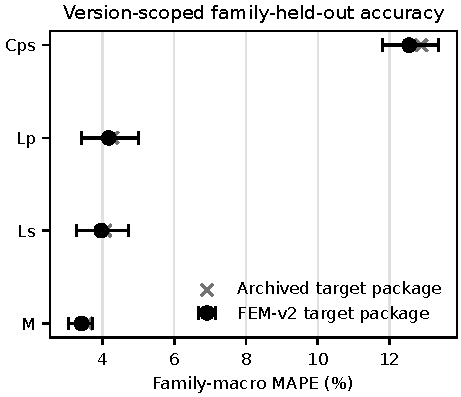
\includegraphics[width=\columnwidth]{hoang4_accuracy.pdf}
\caption{Current and archived target-package results. The marker comparison documents version sensitivity; the two packages are not pooled. Error bars are crossed-axis descriptive sensitivity intervals for the current package.}
\label{fig:accuracy}
\end{figure}

\begin{figure}[!t]
\centering
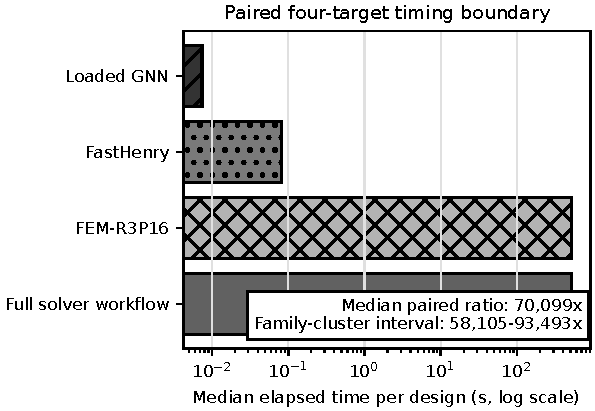
\includegraphics[width=\columnwidth]{hoang7_latency.pdf}
\caption{Median times under the paired all-four-target boundary. The logarithmic axis reveals the FastHenry and FEM components. The paired-ratio statistic is computed per design, not as a ratio of component medians.}
\label{fig:latency}
\end{figure}

The archived 25-thread target package produced mean family-macro errors of 12.890\%, 4.272\%, 4.076\%, and 3.554\%. These values remain an admitted version-scoped result, but the thread-sensitive capacitance generation path means they cannot be relabeled as FEM-v2 evidence. Fig.~\ref{fig:accuracy} retains the earlier central values only as a target-version comparison.

On fixed 39-layout panels per split, the same current-model predictions yield capacitance errors of 12.917\% against FEM-$\Rthree$ and 14.838\% against FEM-$\Rfour$. The five panels contain 195 memberships but only 135 unique layouts from 45 families. This matched view isolates reference fidelity; it does not make R4 truth or the panels independent.

\subsection{Frozen Pooled-Feature Procedures}
Table~\ref{tab:baselines} and Fig.~\ref{fig:baselines} compare the graph model with the four fixed pooled-feature procedures. The GNN has lower family-macro MAPE for all four targets in every matched split/initialization cell against each procedure. All 16 paired descriptive interval endpoints are positive. Because representation and function class change together, the result does not establish a causal advantage of connectivity or superiority over tuned alternatives.

\begin{table*}[t]
\caption{Mean Family-Macro MAPE for the GNN and Frozen Pooled Procedures}
\label{tab:baselines}
\centering
\begin{tabular}{lrrrr}
\toprule
Model & $\Cps$ & $\Lp$ & $\Ls$ & $\Mut$ \\
\midrule
GNN & 12.550 & 4.173 & 3.964 & 3.413 \\
Constant & 62.421 & 71.129 & 68.898 & 57.026 \\
Ridge & 44.480 & 48.666 & 39.522 & 35.826 \\
Random Forest & 42.528 & 36.977 & 39.929 & 33.397 \\
Extra Trees & 42.130 & 30.325 & 39.763 & 29.428 \\
\bottomrule
\end{tabular}
\end{table*}

\begin{figure*}[t]
\centering
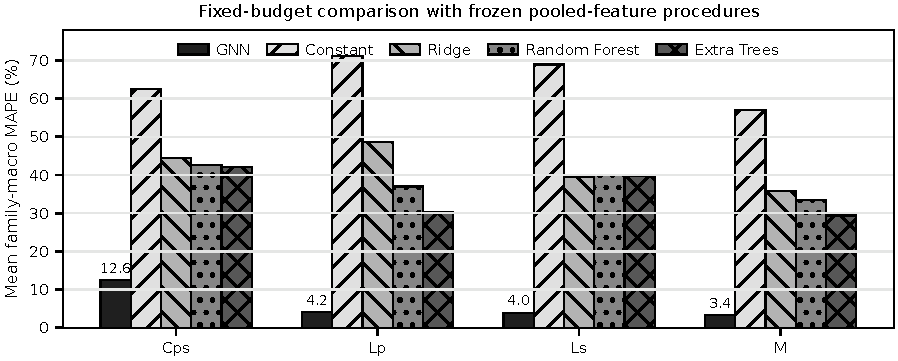
\includegraphics[width=\textwidth]{hoang5_baselines.pdf}
\caption{Mean family-macro MAPE for the GNN and four frozen pooled-feature procedures. Lower is better. The comparison is post-hoc and fixed-budget.}
\label{fig:baselines}
\end{figure*}

\subsection{Coordinate Updates and Symmetry}
The three arms have similar central errors (Table~\ref{tab:coordinate}). Against the same-width control, the coordinate-update arm has lower mean error for $\Cps$, $\Lp$, and $\Ls$ but higher mean error for $\Mut$. Against the approximately parameter-matched control, it has higher mean error for all four targets. The eight moving-minus-fixed descriptive intervals all include zero (Fig.~\ref{fig:coordinate}). The fixed-budget study therefore does not establish a consistent accuracy gain from coordinate updates. It does not establish equivalence, absence of benefit elsewhere, or a universal conclusion about equivariant networks.

\begin{table}[t]
\caption{Coordinate-Update Ablation: Mean Family-Macro MAPE}
\label{tab:coordinate}
\centering
\footnotesize
\begin{tabular}{lrrrr}
\toprule
Arm & $\Cps$ & $\Lp$ & $\Ls$ & $\Mut$ \\
\midrule
Coordinate, width 96 & 11.623 & 4.328 & 4.173 & 3.904 \\
Fixed, width 96 & 11.763 & 4.449 & 4.233 & 3.883 \\
Fixed, matched & 10.895 & 4.269 & 4.090 & 3.810 \\
\bottomrule
\end{tabular}
\end{table}

\begin{figure*}[t]
\centering
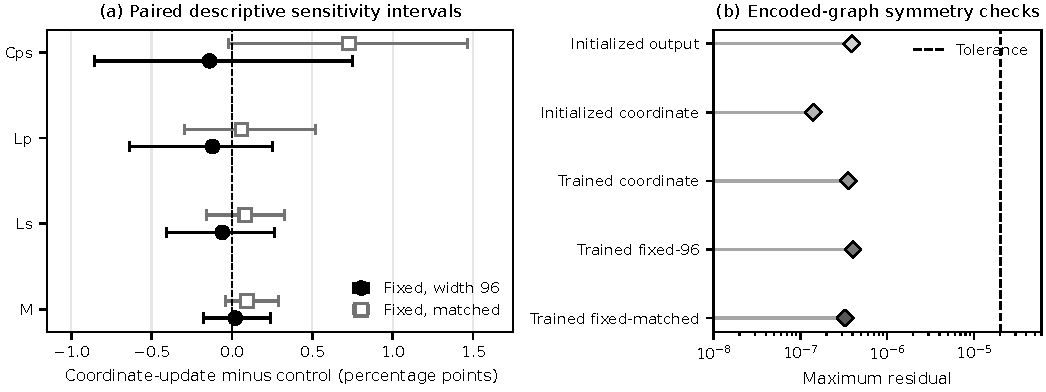
\includegraphics[width=\textwidth]{hoang6_coordinate_symmetry.pdf}
\caption{Coordinate-update study. (a) Moving-minus-fixed paired differences; positive favors the fixed control. All eight descriptive intervals contain zero. (b) Maximum encoded-graph residuals remain below the declared tolerance.}
\label{fig:coordinate}
\end{figure*}

\subsection{Paired Four-Target Runtime}
The timing comparison covers all 306 layouts in split 42, which contains 13 held-out families. One checkpoint, trained with split seed 42 and initialization seed 42, was designated before timing. The GNN timer starts from canonical JSON bytes already resident in memory and includes parsing, geometry validation, graph construction, normalization, batch-one collation, forward computation, inverse target transformation, and materialization of four physical values. The model is already loaded. Each layout receives 50 warm-up calls and 200 measured calls.

The solver timer includes one sequential FastHenry execution for the three inductance targets and one deterministic one-thread FEM-$\Rthree$ execution for capacitance, including input construction, temporary-file handling, solver execution, parsing, numerical checks, and output materialization. It excludes neither solver-internal file operations nor subprocess cost.

For layout $i$, let $g_i$ be its median measured GNN time and $s_i$ its solver-workflow observation. The primary statistic is $\mathrm{median}_i(s_i/g_i)$. Its value is 70,099.076, with a 58,104.638 to 93,493.252 family-cluster descriptive sensitivity interval. Median component times are 7.41936~ms for loaded raw-record-to-four-output GNN inference, 80.96604~ms for FastHenry, 522.90512~s for FEM, and 522.98245~s for the sequential workflow. Capacitance dominates the observed workflow (Fig.~\ref{fig:latency}).

This is not a universal speedup over three-dimensional solvers. It applies to one loaded checkpoint, one CPU class, a resident-input boundary, a fixed one-thread FEM implementation, and one solver observation per design. The descriptive interval does not cover different machines, system load across repeated solver runs, retraining, alternative solvers, or manufactured boards.

\section{Discussion}
The evidence supports three distinct conclusions. First, the GNN approximates the current fixed numerical targets with low single-digit inductance error and a 12.550\% family-macro capacitance error. Second, relational graph prediction is more accurate than the selected frozen pooled-feature procedures on this benchmark, but the comparison does not identify which architectural element causes the difference. Third, imposing coordinate updates supplies a verified symmetry mechanism without an established incremental accuracy benefit under the tested fixed budget.

The capacitance results also show why surrogate error must be interpreted together with reference fidelity. The bulk FEM target passes the tested domain-expansion gate and deterministic repeatability check, yet fails the adjacent-mesh gate. The 198-layout multi-fidelity registry has a same-signed R3-to-R4 discrepancy. A model can reproduce R3 closely while remaining separated from R4, and neither value is fabricated-board truth. Consequently, the paper reports model agreement, numerical-reference discrepancy, and physical-validation status as different quantities.

The current benchmark tests interpolation and family-held-out transfer within one generated geometry system. Holding out complete turn-count families reduces direct template leakage, but materials, board envelope, trace orientation, topology, and active-leg abstraction remain narrow. Commercial component geometry and fabricated-device measurements are separate future validation tracks.

\section{Limitations and Reproducibility}
The corpus excludes routed returns, vias, terminals, planes, ferrite geometry, solder, copper roughness, dielectric anisotropy, and manufacturing variability. FastHenry supplies free-space winding inductance rather than core-inclusive magnetizing behavior. The capacitance references come from one volume-FEM implementation and are not mesh-converged. Higher resolution is a comparator, not ground truth.

The five held-out panels overlap, and the five initialization columns reuse the same split data. Crossed-axis intervals summarize the finite seed grid rather than population coverage. The fixed baseline and coordinate-update studies were designed after earlier GNN results were known. The baseline study is not a tuned-model competition; the coordinate study is not an equivalence test. The runtime study does not quantify cross-machine or solver-run variability.

Reproducibility is provided as a versioned regeneration package rather than a download-and-run physical validation product. The repository freezes geometry contracts, split registries, numerical observations, checkpoints, predictions, summaries, protocol files, and archive manifests. The journal package freezes its claim set, source wiki revision, figure data, generated graphics, bibliography, LaTeX source, and built PDF. External solver builds and substantial compute remain necessary to regenerate the numerical corpus from first principles.

\section{Conclusion}
A credible surrogate requires more than a fast network. This study joins a shared geometry contract, qualified numerical references, family-held-out evaluation, fixed controls, implementation-level symmetry checks, and a paired end-to-end timing boundary. On the current 1,500-layout synthetic benchmark, the graph surrogate achieves 12.550\% capacitance and 3.413 to 4.173\% inductance family-macro error, has lower error than four frozen pooled-feature procedures, and provides four outputs in 7.41936~ms under the measured loaded boundary. A 70,099-fold median paired ratio is observed against the specified sequential numerical workflow. Learned coordinate updates do not show a consistent additional accuracy gain, although their encoded-graph symmetry behavior is verified. The results support numerical-reference screening within the frozen geometry family; extending them to production extraction requires broader routed geometry, stronger mesh evidence, commercial-component transfer, and fabricated-board measurements.

\section*{Acknowledgment}
The authors thank the open-source developers of FastHenry, Gmsh, scikit-fem, PyTorch, and the scientific Python ecosystem used in the reproducible workflow.

\bibliographystyle{IEEEtran}
\bibliography{references}

\end{document}
